\documentclass[a4paper]{article}

%use the english line for english reports
%usepackage[english]{babel}
\usepackage[portuguese]{babel}
\usepackage[utf8]{inputenc}
\usepackage{indentfirst}
\usepackage{graphicx}
\usepackage{verbatim}
\usepackage{float}
\usepackage{listings}

\lstset{emph={%  
   {:-}%
     },emphstyle={\color{red}\bfseries\underbar}%
}%


\begin{document}

\setlength{\textwidth}{16cm}
\setlength{\textheight}{22cm}

\title{\Huge\textbf{\textit{Crab Stack}}\linebreak\linebreak\linebreak
\Large\textbf{Relatório Intercalar}\linebreak\linebreak
\linebreak\linebreak

\includegraphics[scale=0.1]{feup-logo.png}\linebreak\linebreak
\linebreak\linebreak
\Large{Mestrado Integrado em Engenharia Informática e Computação} \linebreak\linebreak
\Large{Programação em Lógica}\linebreak
}

\author{\textbf{Grupo Crab\textunderscore Stack\textunderscore 1:}\\
Inês de Sousa Caldas - up200904082 \\
Maria Teresa Chaves - up201306842 \\
\linebreak\linebreak \\
 \\ Faculdade de Engenharia da Universidade do Porto \\ Rua Roberto Frias, s\/n, 4200-465 Porto, Portugal \linebreak\linebreak\linebreak
\linebreak\linebreak\vspace{1cm}}

\maketitle
\thispagestyle{empty}

%************************************************************************************************
%************************************************************************************************

\newpage

%%%%%%%%%%%%%%%%%%%%%%%%%%
\section{O Jogo \textit{Crab Stack}}

O jogo \textit{Crab Stack} foi publicado pela \textit{Blue Orange Games} em 2015. Este foi conceptualizado por \textit{Henri Kermarrec} que contou com a colaboração da artista \textit{Stéphane Escapa}. Enquadra-se nas categorias de jogos abstratos e familiares, sendo aconselhado a jogadores com idade superior a 8 anos\footnote{http://www.geekyhobbies.com/crab-stack-review-and-instructions/}.

Este jogo pode ser jogado por dois a quatro jogadores. Dependendo do número de jogadores apenas uma parte do tabuleiro é utilizado. No caso de serem dois jogadores utiliza-se apenas as rochas amarelas (figura \ref{Fig:tabuleiro}); no caso de serem três jogadores, para além das rochas amarelas também são utilizadas as rochas pretas; e por último no caso de serem quatro jogadores, joga-se em todo o tabuleiro\footnote{http://www.blueorangegames.com/index.php/games/crab-stack}. No contexto da unidade curricular de Programação em Lógica, é pretendido o desenvolvimento de um jogo de tabuleiro para dois jogadores. Desta forma apenas serão enunciadas as regras\footnote{https://boardgamegeek.com/boardgame/172033/crab-stack} relacionadas com o modo de dois jogadores.

\begin{figure}[!ht]
	\begin{center}
	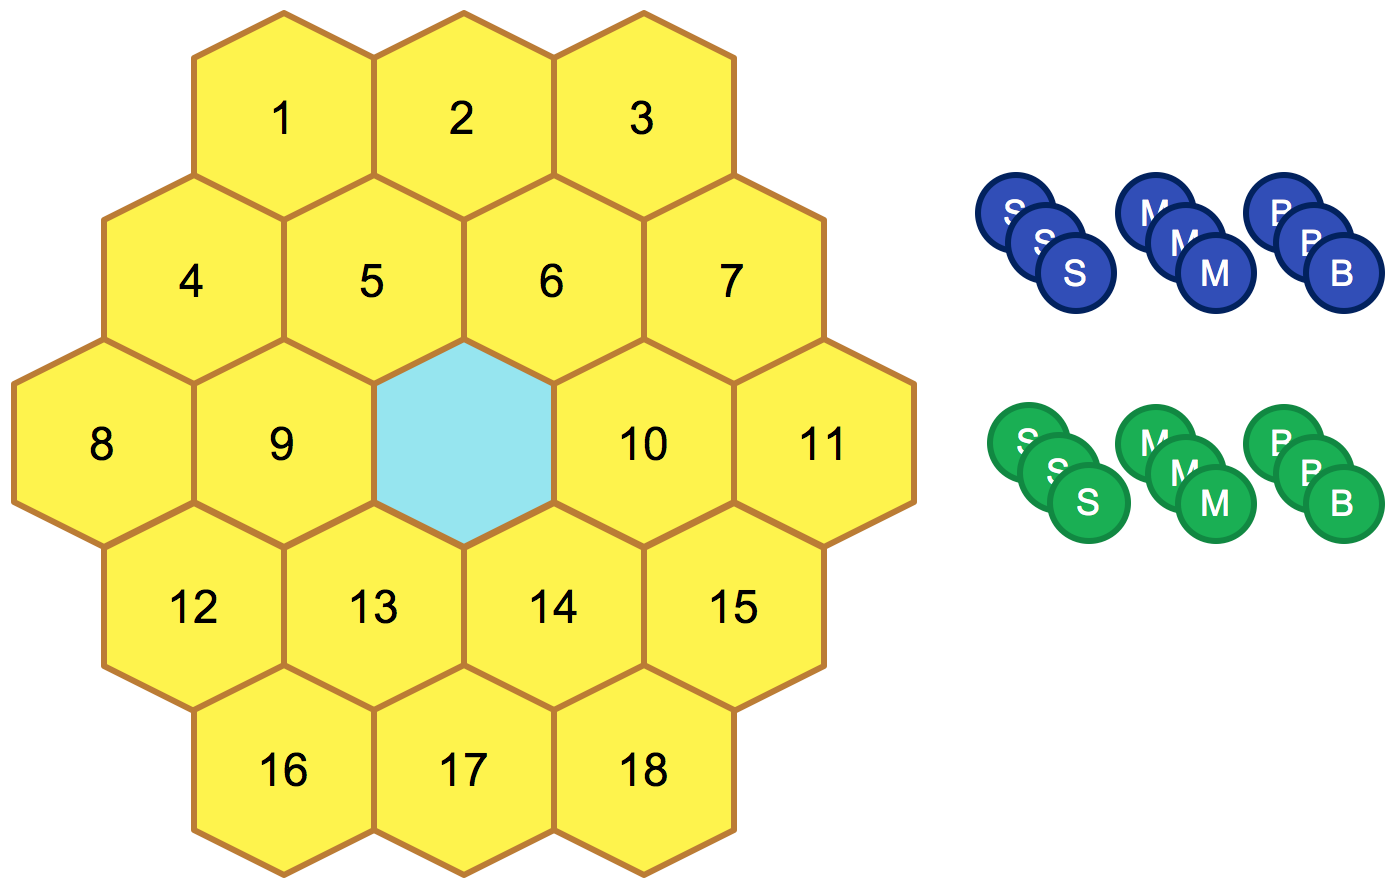
\includegraphics[scale=0.4]{board.png}
	\caption{Tabuleiro de jogo}
    \label{Fig:tabuleiro}
	\end{center}
\end{figure}

\subsection{Preparação do tabuleiro}

Com um formato hexagonal, o tabuleiro é formado por 18 posições, como é possível observar na figura \ref{Fig:tabuleiro} nas rochas amarelas.
\newline
A cada jogador é atribuído um conjunto de 9 caranguejos: 3 grandes, 3 médios e 3 pequenos, como é possível observar no lado direito da figura \ref{Fig:tabuleiro}.
\newline
Antes do jogo começar, os caranguejos dos jogadores são distribuídos aleatoriamente pelo tabuleiro obedecendo às regras de empilhamento que serão explicitadas na secção \ref{movimentos_caranguejo}.

\subsection{Movimentos possíveis} \label{movimentos_caranguejo}

No turno de um jogador, este pode mover um dos seus caranguejos de forma a terminar o seu movimento numa rocha ocupada por outro caranguejo. Dependendo do seu tamanho, um caranguejo move-se, obrigatoriamente, um determinado número de rochas:
\begin{itemize}
\item Pequeno - move-se três rochas;
\item Médio - move-se duas rochas;
\item Grande - move-se uma rocha.
\end{itemize}
No final do movimento, um caranguejo não pode regressar à rocha inicial.
\newline
Apenas os caranguejos que estejam no topo da pilha podem ser movidos durante o turno de um jogador.
\newline
O empilhamento dos caranguejos tem de obedecer às seguintes regras:
\begin{itemize}
\item um grande pode ficar em cima de qualquer outro caranguejo;
\item um médio pode ficar em cima de um caranguejo médio ou pequeno;
\item um pequeno pode apenas ficar em cima de outro caranguejo pequeno.
\end{itemize}

\subsection{Regra da Onda}
Os caranguejos gostam de estar em grupos grandes e não gostam de ser separados. Numa situação em que os caranguejos fiquem separados em dois grupos, por uma linha de rochas vazias, um destes grupos irá ser eliminado do jogo por uma onda. O grupo a ser eliminado é selecionado pela seguinte ordem de prioridades:
\begin{enumerate}
\item O grupo de caranguejos que ocupar menos espaço no tabuleiro é removido do jogo;
\item Se os dois grupos ocupam o mesmo número de casas no tabuleiro, então o grupo com o menor número total de caranguejos é removido do jogo;
\item Se o número de caranguejos for o mesmo, o jogador do turno em que ocorreu a separação, decide qual o grupo que irá ser removido do jogo.
\end{enumerate}

\subsection{Fim do jogo}

O \textit{Crab Stack} pode terminar nos seguintes estados do jogo:
\begin{itemize}
\item Se todas as peças de um jogador forem removidas do jogo, através de uma onda, o jogador perde o jogo;
\item Se um jogador, no inicio do seu turno, não conseguir mover nenhum dos seus caranguejos, perde o jogo;
\item Caso o jogo chegue a um ponto em que os jogadores estão repetidamente a executar os mesmos movimentos, o jogo termina e ocorre um empate. Desta forma, é necessário realizar um novo jogo para determinar o vencedor do jogo.
\end{itemize}

%%%%%%%%%%%%%%%%%%%%%%%%%%
\newpage
\section{Representação do Estado do Jogo}

\subsection{Representação do estado do tabuleiro}

O tabuleiro é representado por uma lista de listas, em que cada elemento da lista representa uma rocha. Os caranguejos de cada jogador serão representados por Sx, Mx, Bx, em que x representa o número do jogador e S, M, B o tamanho do caranguejo, respetivamente pequeno, médio e grande. Uma rocha, i.e. uma célula da lista, tem dois estados diferentes possíveis: estar vazia ou ter uma pilha de caranguejos. Uma pilha de caranguejos, pode ser por exemplo [B1, S1, S2], em que o elemento B1 representa o topo da pilha.
\\O código para a criação de um tabuleiro é dado por:

\begin{lstlisting}[language=Prolog]
make_board(-Board, +NumPlayers):-
	NumPlayers == 2,
	% for other number of players, only the number of lines
	% and  the size change
	Size is 3,
	Line is 5,
	make_board_aux(-Board,[], +Line, +Size).
\end{lstlisting}

\subsection{Posições iniciais do jogo}

No início do jogo, as peças de cada jogador são colocadas aleatoriamente no tabuleiro, garantindo que fica com todas as rochas ocupadas. Abaixo segue-se o predicado que inicia o jogo e um exemplo de um tabuleiro no estado inicial do jogo.
\begin{lstlisting}[language=Prolog]
init_crabs(-FinalBoard, +Board, +Crabs).
Board =  [ %initial board example
    	 	[[S1][M2][M1]]
         	[[B2][B1][M1][S2]]
         	[[S2][S1][W][M2][B2]]
    	 	[[M2][B2][S1][B1]]
    	 	[[M1][S2][B1]]
    	 ]
     
\end{lstlisting}

Para uma melhor visualização do estado inicial representado acima, segue-se uma figura ilustrativa.

\begin{figure}[!ht]
	\begin{center}
	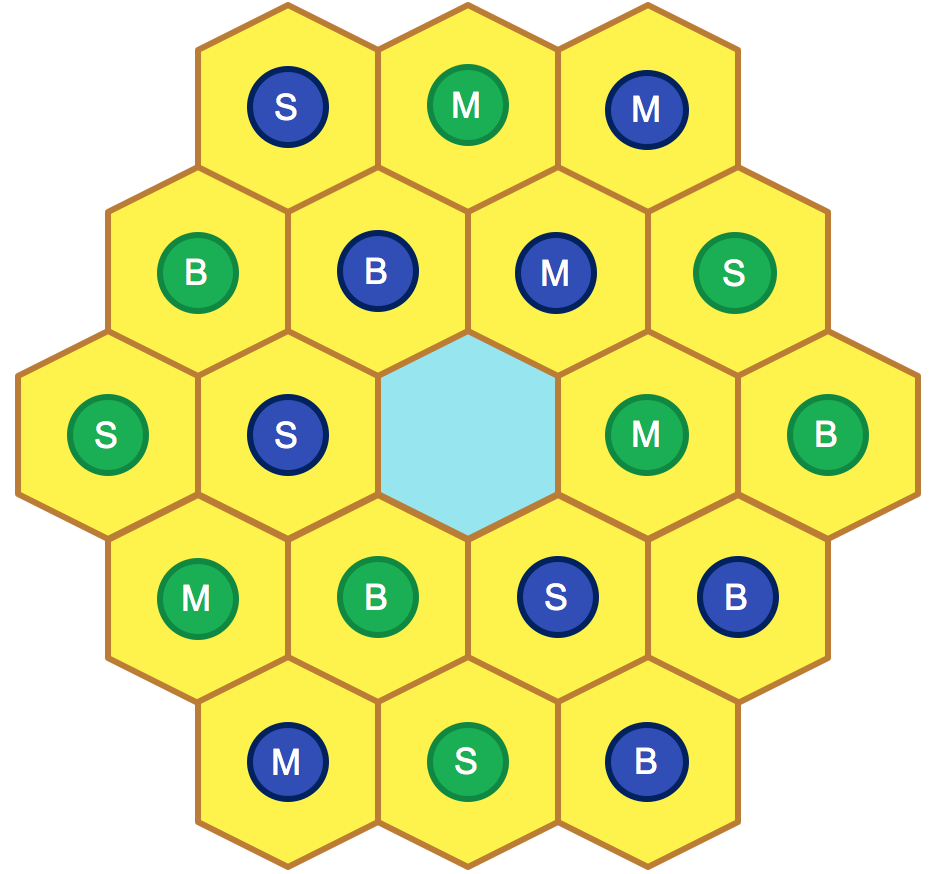
\includegraphics[scale=0.29]{init_board.png}
	\caption{Estado inicial do jogo}
    \label{Fig:tabuleiro_inicial}
	\end{center}
\end{figure}

\newpage

\subsection{Posições intermédias do jogo} \label{section:intermedia}

Abaixo seguem-se exemplos de tabuleiros num estado intermédio do jogo.

\begin{lstlisting}[language=Prolog]

Board =  [%General Intermediate state board
    	 	[[M1,M2,S1][][]]
         	[[][B1][M1][S2]]
         	[[B2,S2][S1][W][M2][B1,B2]]
    	 	[[B2,M2][][B1,S1][]]
    	 	[[][M1,S2][]]
     	 ]
         
Board =  [% Intermediate state board With a possibility for a wave
    	 	[[][S1][M1]]
         	[[B2][M1][B1][S2]]
         	[[][S2][W][B1,M2][B1,B2]]
    	 	[[M1,M2][S1][][S2,S1]]
    	 	[[B2][M2][]]
     	 ]
         
Board =  [% Intermediate state board ready for the Wave
    	 	[[][M1,S1][M1]]
         	[[B2][][B1][S2]]
         	[[][S2][W][B1,M2][B1,B2]]
    	 	[[M1,M2][S1][][S2,S1]]
    	 	[[B2][M2][]]
     	 ]
         
Board =  [% Intermediate state board after the Wave
    	 	[[][M1,S1][M1]]
         	[[][][B1][S2]]
         	[[][][W][B1,M2][B1,B2]]
    	 	[[][][][S2,S1]]
    	 	[[][][]]
     	 ]
\end{lstlisting}

Para uma melhor visualização da regra da onda, seguem-se imagens ilustrativas do exemplo apresentado acima, com os diferentes estados intermédios.

\begin{figure}
\begin{tabular}{cc}
  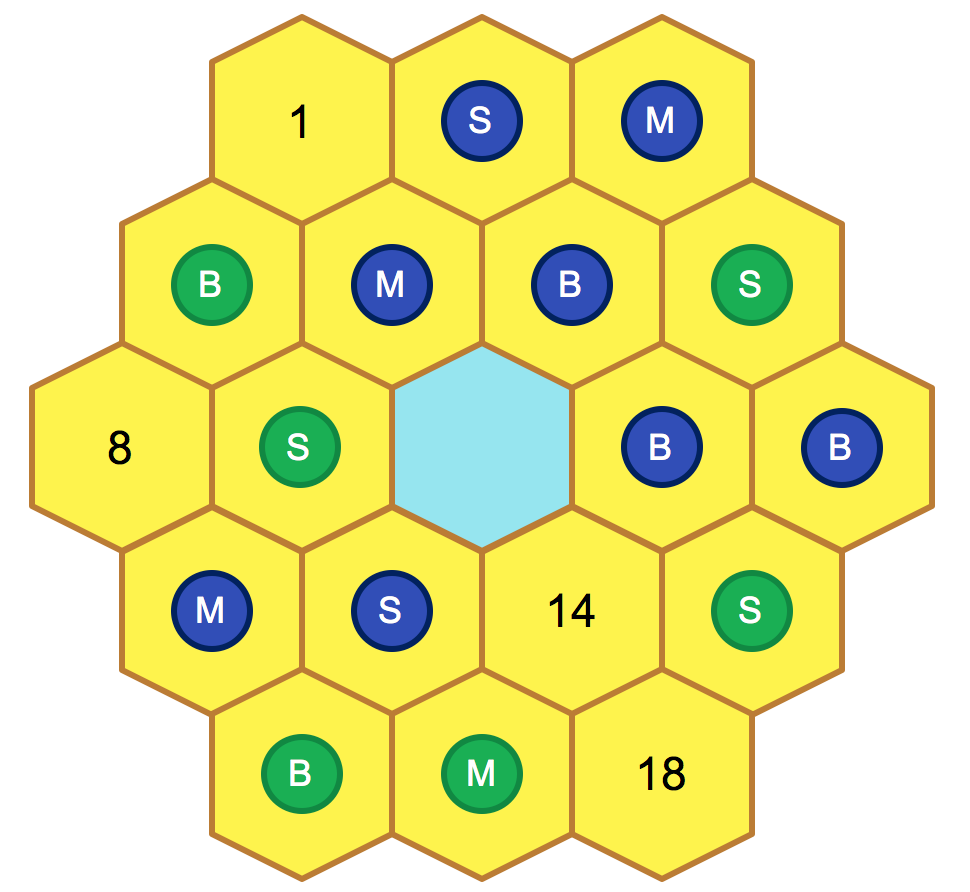
\includegraphics[width=55mm]{wave1.png} &   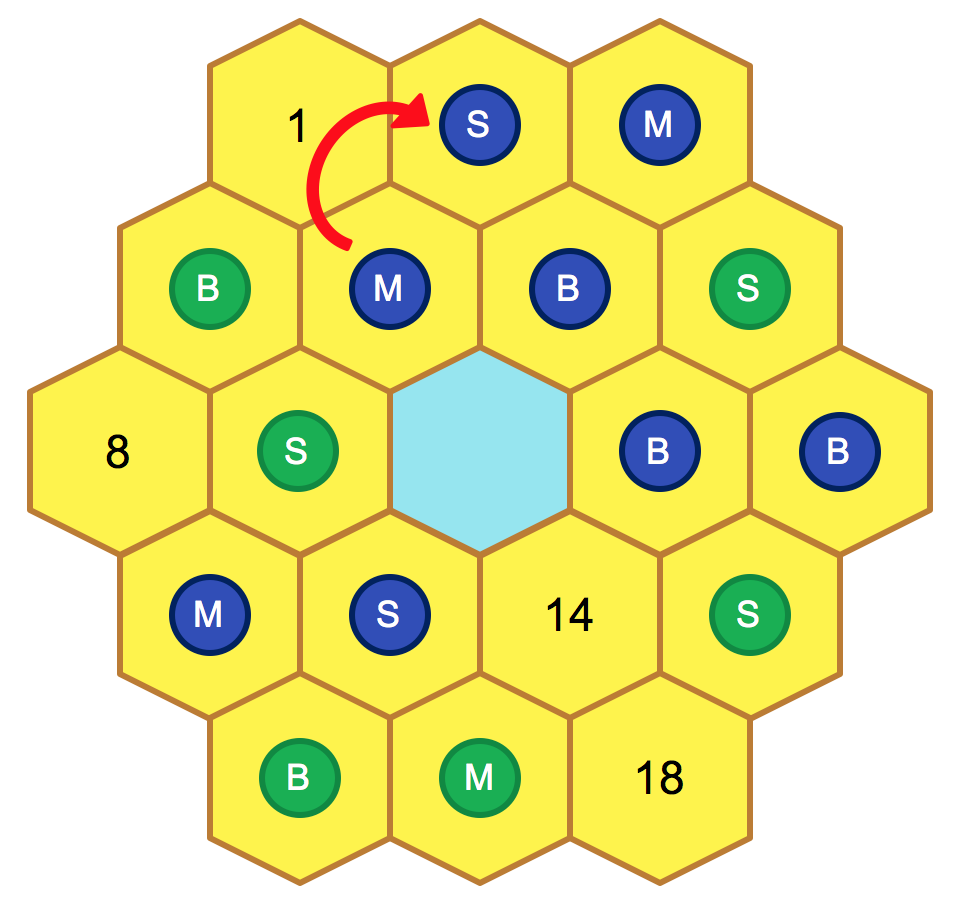
\includegraphics[width=55mm]{wave2.png} \\
(a) Possibilidade de ocorrer uma onda. & (b) Jogador azul move peça para  ocorrer uma onda. \\[6pt]
 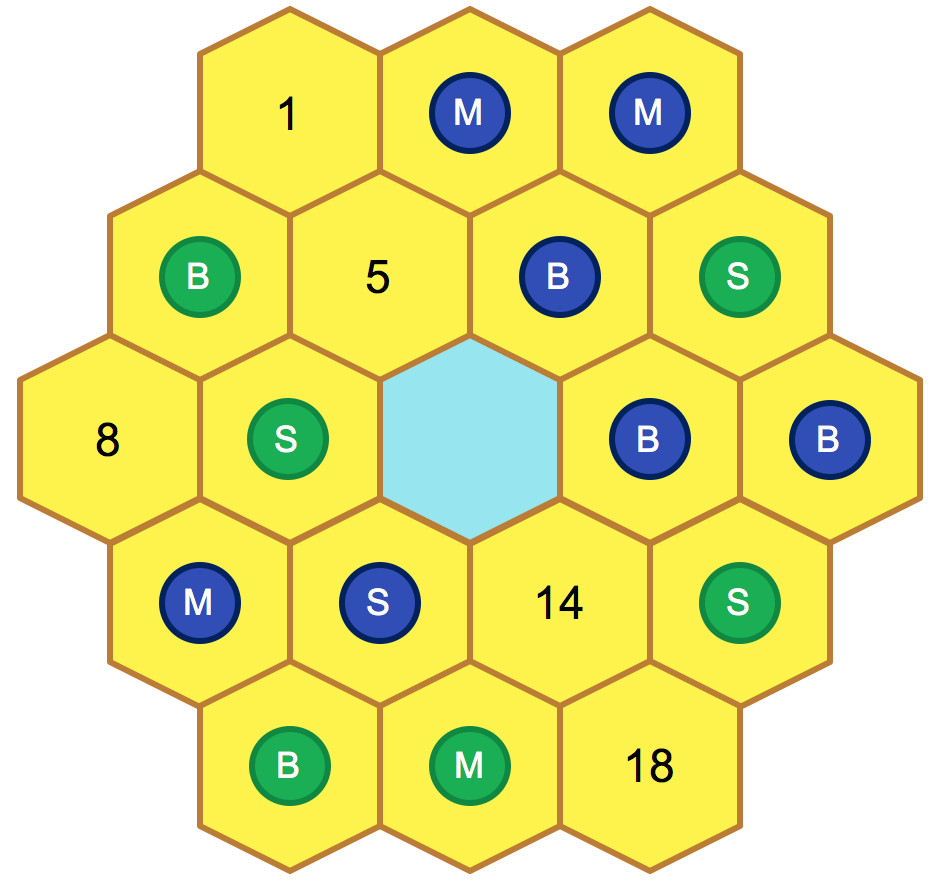
\includegraphics[width=55mm]{wave3.png} &   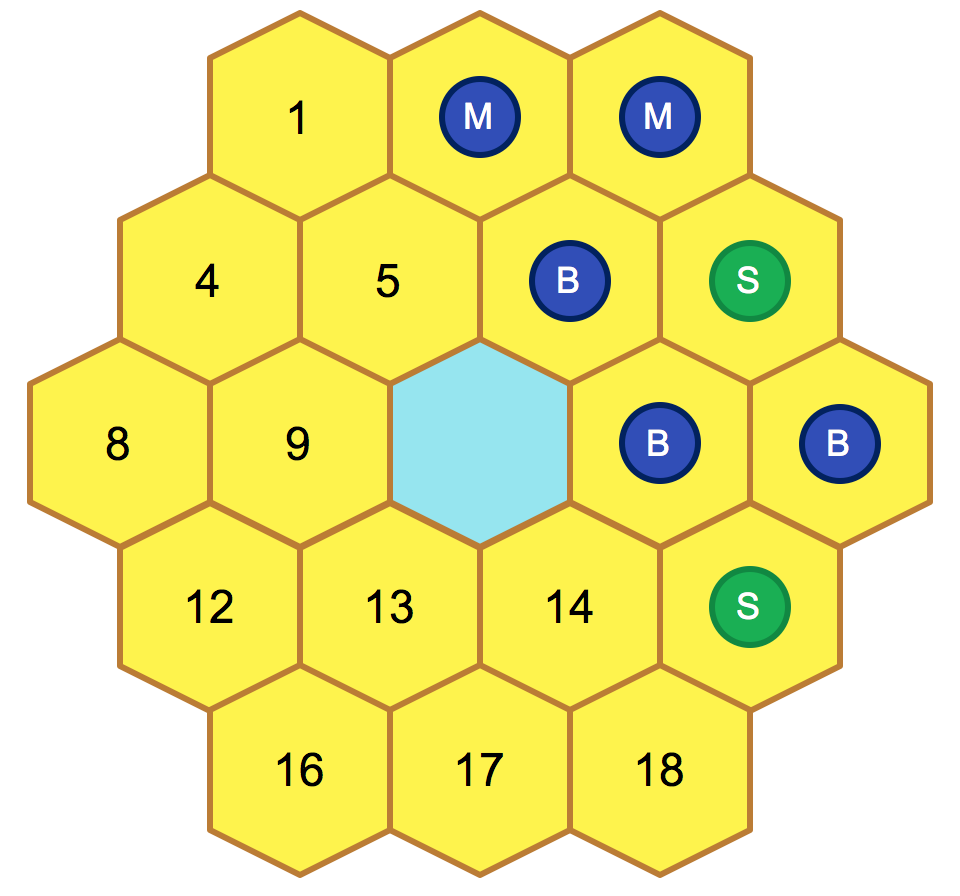
\includegraphics[width=55mm]{wave4.png} \\
(c) Ocorre uma onda. & (d) Peças do grupo esquerdo são removidas do jogo. \\[6pt]
\multicolumn{2}{c}{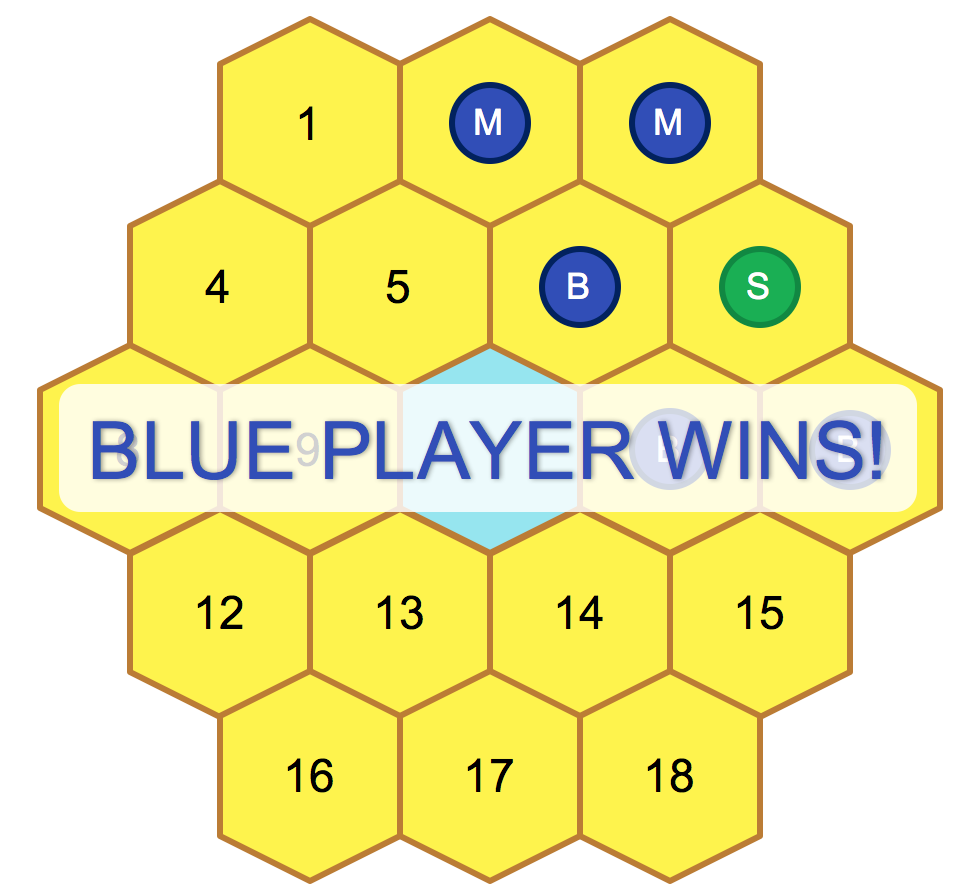
\includegraphics[width=55mm]{end_game.png} }\\
\multicolumn{2}{c}{(e) O jogador azul ganha o jogo.}
\end{tabular}
\caption{Exemplo da ocorrência de uma onda durante o turno do jogador azul.}
\label{fig:intermedia}
\end{figure}

\newpage

\subsection{Posições finais do jogo}

No exemplo da onda, mencionada na secção anterior, verifica-se que após a onda, o jogador verde apenas pode mover um dos seus caranguejos pequenos para cima do seu outro caranguejo pequeno, deixando de ter movimentos possíveis, e portanto o jogador azul ganha o jogo.
\begin{lstlisting}[language=Prolog]

Board =  [% Green's turn after the wave
    	 	[[][M1,S1][M1]]
         	[[][][B1][S2]]
         	[[][][W][B1,M2][B1,B2]]
    	 	[[][][][S2,S1]]
    	 	[[][][]]
     	 ]
         
Board =  [% Final state board after the green's move
    	 	[[][M1,S1][M1]]
         	[[][][B1][S2,S2]]
         	[[][][W][B1,M2][B1,B2]]
    	 	[[][][][S1]]
    	 	[[][][]]
     	 ]
\end{lstlisting}

%%%%%%%%%%%%%%%%%%%%%%%%%%
\section{Visualização do Tabuleiro} 

Para a visualização do tabuleiro, irão ser implementados os seguintes predicados:
\begin{itemize}
\item Cabeçalho do predicado para a visualização do tabuleiro:
\begin{lstlisting}[language=Prolog]
display_board(+Board).
\end{lstlisting}
\item Cabeçalho do predicado para a visualização da pilha:
\begin{lstlisting}[language=Prolog]
display_stack(+Rock, +Stack).
\end{lstlisting}
\end{itemize}

Segue-se a visualização do output do predicado \textit{display\textunderscore board} para o primeiro exemplo de um estado intermédio de jogo apresentado na secção \ref{section:intermedia}.

\begin{figure}[!ht]
	\begin{center}
	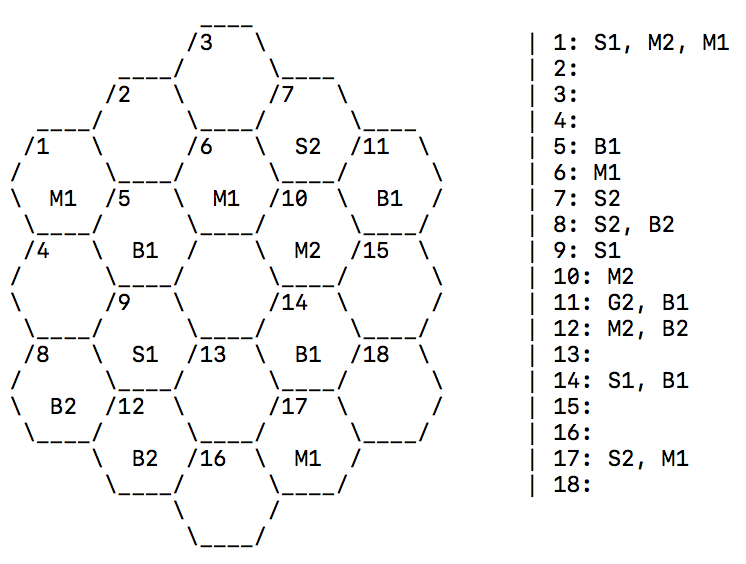
\includegraphics[scale=0.4]{display_board.png}
	\caption{Representação do output no estado intermédio do jogo.}
    \label{Fig:display_board}
	\end{center}
\end{figure}

%%%%%%%%%%%%%%%%%%%%%%%%%%
\newpage
\section{Movimentos}

Para os movimentos existentes no \textit{Crab Stack}, explicados na secção \ref{movimentos_caranguejo}, serão implementados os seguintes predicados:

\begin{itemize}
\item Cabeçalho do predicado para o movimento de um caranguejo:
\begin{lstlisting}[language=Prolog]
moveCrab(-FinalBoard, +Board, +CrabSize, +PosInit, +PosFinal).
\end{lstlisting}
\item Cabeçalho do predicado para a verificação da ocorrência de uma onda:
\begin{lstlisting}[language=Prolog]
checkWave(-FinalBoard, +Board).
\end{lstlisting}
\item Cabeçalho do predicado para a verificação do fim do jogo, i.e., a impossibilidade de movimentos por parte de um dos jogadores:
\begin{lstlisting}[language=Prolog]
checkMoves(-Winner, +Board).
\end{lstlisting}
\end{itemize}


\end{document}
